\chapter{An Overview of Snapstore}

Snapstore was created with two distinct groups of users in mind, non-technical users and technical users. In order to be an attractive system to technical users who use systems like Git, Snapstore needed to support the functionality of powerful version control systems. However, Snapstore also needed to have a smoother learning curve to promote quick startup and attract users who feel overwhelmed by complicated VCSs. 

We decided to create Snapstore with an opt-in strategy concerning complexity. Users can download Snapstore and get started right away with simple actions like file backup. Then, if desired, users can explore more advanced features of the system.

%Snapstore uses a simple user-based identification system. Once a user downloads Snapstore, they create an account with a username.

Snapstore operates within a specially designated Snapstore folder which is created upon opening the application for the first time. It is similar to the Dropbox folder; Snapstore only looks at files that are inside of it. Snapstore watches the user's filesystem for changes in order to respond with certain actions like creating snapshots (section 2.1.1). This allows users to use any editor with Snapstore. Also, the Snapstore folder that Snapstore creates does not need to remain the only folder used by the application. Snapstore can be opened using any folder as the Snapstore folder.

\section{Basic Features}

The basic features of Snapstore allow a single user to use the application like they would a file syncing system.

\subsection{Snapshots}

\textit{Snapshots} allow a user to persistently store all of their edits to a file over time. Whenever a file is saved to disk, a snapshot is created with the contents of that file and stored in the local repository. The type of each snapshot corresponds to the action that created it. Snapshots can be the result of a create, update, rename, delete, merge, or conflicting merge of a file. Users can retreive an old state of a file by finding the appropriate snapshot in the file's history.

Snapshots are created when a file is created, updtaed, deleted or renamed. Snapshots are also created when files are merged together. These snapshots are either the result of a successful merge or of a conflicting merge. Snapshots, then, can be one of six types: create, update, delete, rename, merge, or conflict.

When creating snapshots for a given file, Snapstore will add the snapshot to that file's \textit{snapshot graph}. This graph represents the history of the file and it shows each snapshot that was taken, along with its relationship to other snapshots of that file. A snapshot has one or more parents (the snapshot(s) taken before it), and it has a child (the snapshot taken after it). The only way a snapshot could have more than one parent is if it's a product of a merge of multiple snapshots. The first snapshot in a graph is called the \textit{root}, and the last snapshot in the graph is called the \textit{head}.

To show a sequence of snapshots from a file's history, navigate to that file within Snapstore's interface. Then, click on the file's name. The snapshot graph will appear at the top of the window. Each node in this graph is a snapshot, and the node on the far right is the head. By clicking on these nodes, the content of the snapshot will appear on the bottom-right of the window. After the correct snapshot is found, it's possible to revert to that snapshot by clicking ``Revert'', a button above the snapshot content. Reverting to a previous snapshot will create a new snapshot with the same content at the head position and alter the file's content to match the snapshot's content.

\subsection{Upstreams}

\textit{Upstreams} are used to synchronize the data of collaborators on a project. Whenever a user makes any changes to their Snapstore system, those changes are sent to the upstream and out to all other users who are collaborating with that user.

If two users are working together on a project, the upstream will synchronize their snapshots as they make them. In the case of multiple snapshots coming in to the upstream at the same time, the upstream will resolve the conflict and push the same ordering of snapshots to both users.

By default, the upstream is the Snapstore server, but users might want to change their upstream so their data passes through a known location. To do so, follow these steps:
\begin{enumerate}
  \item{Download the Snapstore server program onto the machine}
  \item{Run the Snapstore server on that machine}
  \item{Point the Snapstore client to that machine}
\end{enumerate}

\subsection{Local Repository}

The \textit{local repository} allows users to work without an active Internet connection. Whenever a user makes any changes to their Snapstore system that data is saved in the local repository. When connection is restored, Snapstore will push all new changes to the upstream.

\section{Advanced Features}

Snapstore's advanced features allow users to access the more powerful components of a version control system. They provide additional functionality that users might want when working on projects with complex version control requirements.

\subsection{Groups}

\textit{Groups} allow users to designate a collection of snapshots as related. When a user has a collection of snapshots they believe are related, even if they exist across multiple files, they can place them in a group. The user can then give this group a name.

A software team collaborating on a project might want to fix a syntax bug in their program. If one user makes a few snapshots in this process, they can then place them in a group and title it ``Fixed syntax bug''. Now, these snapshots and this group have all been shared with the other team members through the upstream. Team members can easily locate this group and inspect its snapshots to see how the bug was fixed. 

\subsection{Tags}

\textit{Tags} allow users to designate a group as a coherent point in development. The exact nature of a coherent point will differ from project to project, but in general this means a point in which the project is ready for further development. When a group of snapshots is particularly significant, such as project completion or a release of a piece of software, users can tag that group.

Tags can only be given to groups who have at most once snapshot per file. This is so that a the user can revert the state of their files using the tag. When this is done, every file that is in the group with that tag will be reverted to the state described by the snapshots in that group.

For a software release, a user can tag the group of head snapshots ``Version 1.3'' to signify that the project is in a stable release state. Later, after more snapshots have been created, users can utilize this tag to revert the project to the group of snapshots tagged by ``Version 1.3''.

\subsection{Branches}

\textit{Branches} allow users to separate parallel lines of work. Whenever any data is created, it is saved within the user's current branch. Switching to a different branch will load all data associated with that branch, changing the user's filesystem as necessary. Branches can be merged together to combine parallel lines of work.

Snapstore provides a default branch called ``master'' on startup. A user can then create and use new branches to maintain multiple versions/releases of the same project, keep the development of major features isolated, and to give users the ability to try out experimental changes without affecting the main line \cite{RossoJackson}.

A branch can also be created by cloning an existing branch. Creating a clone involves choosing a branch to clone and selecting snapshots inside the original branch to bring over to the clone. For all snapshots that are cloned into the new branch, any groups associated those snapshots, and any tags associated with those groups, will be copied to the cloned branch.

\subsubsection{Sharing Branches}

When a branch is shared with another user, that branch's data is copied on that user's local repository. On a shared branch, when any user makes changes, those changes are immediately sent to the other user(s) associated with that shared branch. For example, one user might create a new snapshot on a file in the shared branch. That new snapshot is propagated to all collaborators on that branch and reflected in their snapshot graphs and on their filesystem.

When conflicts arise due to multiple users working on the same branch at the same time, Snapstore uses last-write wins rule. The last snapshot to reach the server will become the head snapshot for the file. Other snapshots are placed before the head snapshot in the snapshot graph. No snapshots are lost in the conflict, and the user can revert to a passed over snapshot easily.

Figure 2-1 illustrates an example of two user working on a shared branch. When two snapshots are created at the same time, one will reach the upstream first. When this happens, that snapshot is confirmed and cannot be changed. When the second snapshot reaches the upstream, it will be rejected. Any snapshots that caused the rejection will be returned with the rejection to be inserted into the user's snapshot graph. The snapshot is then sent again and, if it successfully added to the upstream, it will be sent to all collaborators on that branch.

\begin{figure}
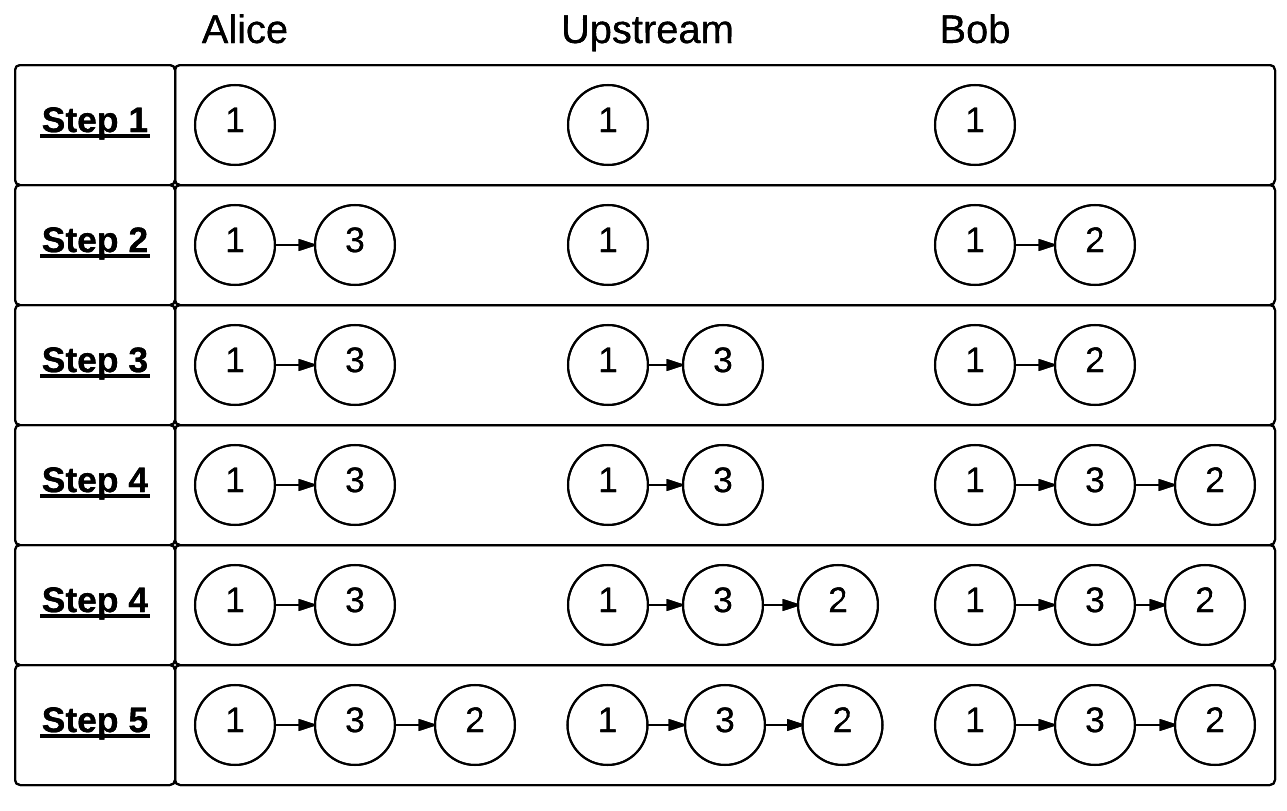
\includegraphics[max width= \linewidth]{Collaborating}
\caption{Conflicts being resolved on a shared branch.}
\label{arm:fig1}
\end{figure}

\subsubsection{Merging Branches}

Merging two branches compares the snapshot graphs in those two branches. If two snapshot graphs correspond to the same file, then a merge is performed using three way merge and their common ancestor. This will result in a merge snapshot with as many parents as there are snapshots being merged. If there is a merge conflict, then the resulting snapshot will be a conflict snapshot. Like in Git, a conflict snapshot's content will show where the conflict needs to be resolved. Unlike in Git, this merge snapshot is already on the server and saved, no conflict resolution is needed to continue working. By simply fixing the conflict and saving, a new snapshot is created that reflects the fix. Merging two branches will keep all of the group and tag data from both branches.

Figure 2-2 shows an overview of branch merging in Snapstore. In this image, the file id is shown next to the head snapshot for each snapshot graph. Once snapshot graphs are identified as corresponding to the same file id, their head snapshots are merged into a new snapshot, whose parents are the old head snapshots. Any snapshot graph that does not have a counterpart in the other branch will just be copied over to the merged branch.

\begin{figure}
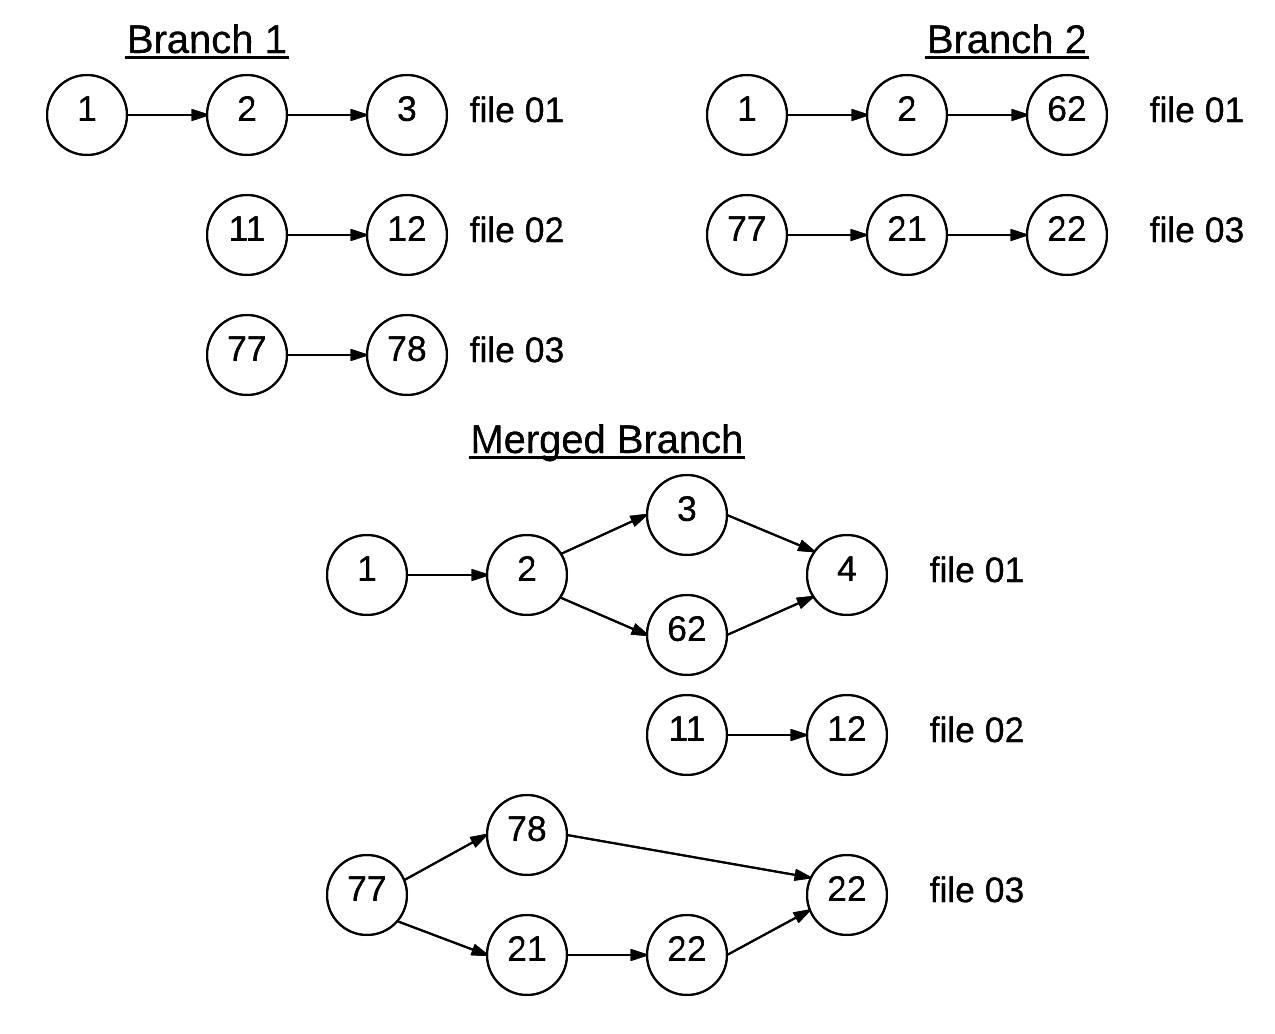
\includegraphics[max width= \linewidth]{Merging}
\caption{Merging two branches.}
\label{arm:fig1}
\end{figure}

\subsection{Use Cases}

\subsubsection{Single User on Multiple Computers}

Git users can sympathize with the hassle of having to commit, push and then pull whenever changing computers. Snapstore solves this using upstreams and local repositories.

Imagine the a user has two computers, $A$ and $B$. Both have a file called ``foo.txt'' on them. The user works on computer $A$, making edits to ``foo.txt''. These changes are saved to their local repository. When they open Snapstore on computer $B$, computer $A$'s local repository will push those changes to computer $B$ through the upstream. Now, computer $B$ has an updated version of ``foo.txt'' that has the exact same content as ``foo.txt'' on computer $A$. There is no push/pull model in Snapstore. Data is automatically propagated to every local repository that has access to the data.

\subsubsection{Project Partitioning and Re-Assembly}

Snapstore uses branches to allow users to partition their projects; they can they distribute these partitions to other users. This helps manage projects, and it can produce powerful workflows. Snapstore can achieve a workflow similar to that used by the Linux project and its system of trusted lieutenants who vet incoming contributions before passing them on to the project owner \cite{linux}.

Imagine that a website is be developed called ``Iweb''. The team creating this website has a project manager, a back-end developer, and a front-end developer. There is a master branch, ``Iweb-master'', that the project manager has access to. In order to partition this project, the project manager makes two clones of this branch, ``Iweb-front'' and ``Iweb-back''. She then shares ``Iweb-back'' with the back-end developer and ``Iweb-front'' with both the front and back-end developer.

A graphical representation of these branches, along with who has access to them, is included in figure 2-3.

\begin{figure}
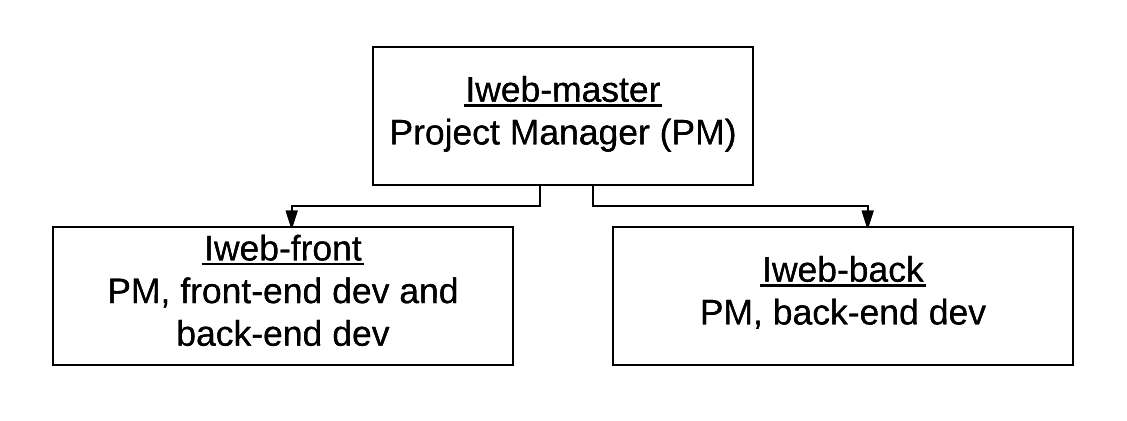
\includegraphics[max width= \linewidth]{caseStudy}
\caption{Icorp's branch hierarchy.}
\label{arm:fig1}
\end{figure}

When edits are made by the developers, they are immediately seen by the project manager because they share the same branch. When the project manager decides that a certain branch, like ``Iweb-front'', is in a stable state, they can merge it with ``Iweb-master''.

This hierarchy of branches accomplishes two things. First, it allows the project manager to vet edits to the cloned branches before merging them onto the master branch. Second, it allows some work to be hidden from some employees, achieving effective access control. The front-end developer does not have access to any of the files in ``Iweb-back''.

This hierarchy of branches can be expanded, allowing Snapstore to achieve a workflow similar to that of very large software projects, such as Linux. 




